\subsection{Studies in the Highly Restricted Phase Space} % (fold)
\label{sub:small_window_studies}

Removing the discrimination power of $\tau_{21}$ and the jet mass in Sec.~\ref{sub:flat_hypercube_studies} allowed us to quantify the unique discrimination power learned by the neural networks.  However, it does not tell us what information is learned.  Another way to quantify the unique information learned by the network that also provides useful information about physical information learned by the network is to restrict the considered phase space such that $\tau_{21}$ and the jet mass distributions do not vary appreciably over the redacted space.  

Though we see performance improvements using a deep network under an induced flat hypercube, we want to be sure that these performance improvements are valid and carry over to a less contrived distribution. In particular, we consider a mass window of [79, 81] GeV, a $p_T$ window of [250, 255] GeV, and we require $\tau_21$ to be in [0.19, 0.21]. In Figure~\ref{fig:meanImagesWindow}, we see the differences between signal and background for such a window.




In this window, we compare the DNN trained outside the window to a Fisher Linear Discriminant trained inside the window. In Figure~\ref{fig:rocWindow} we see this performance comparison, and note that our DNN outperforms the FLD.

\begin{figure}[bt]
  \begin{center}
  
      \subfloat[Average $W'\rightarrow WZ$ image \label{subfig:sig_window}]{
        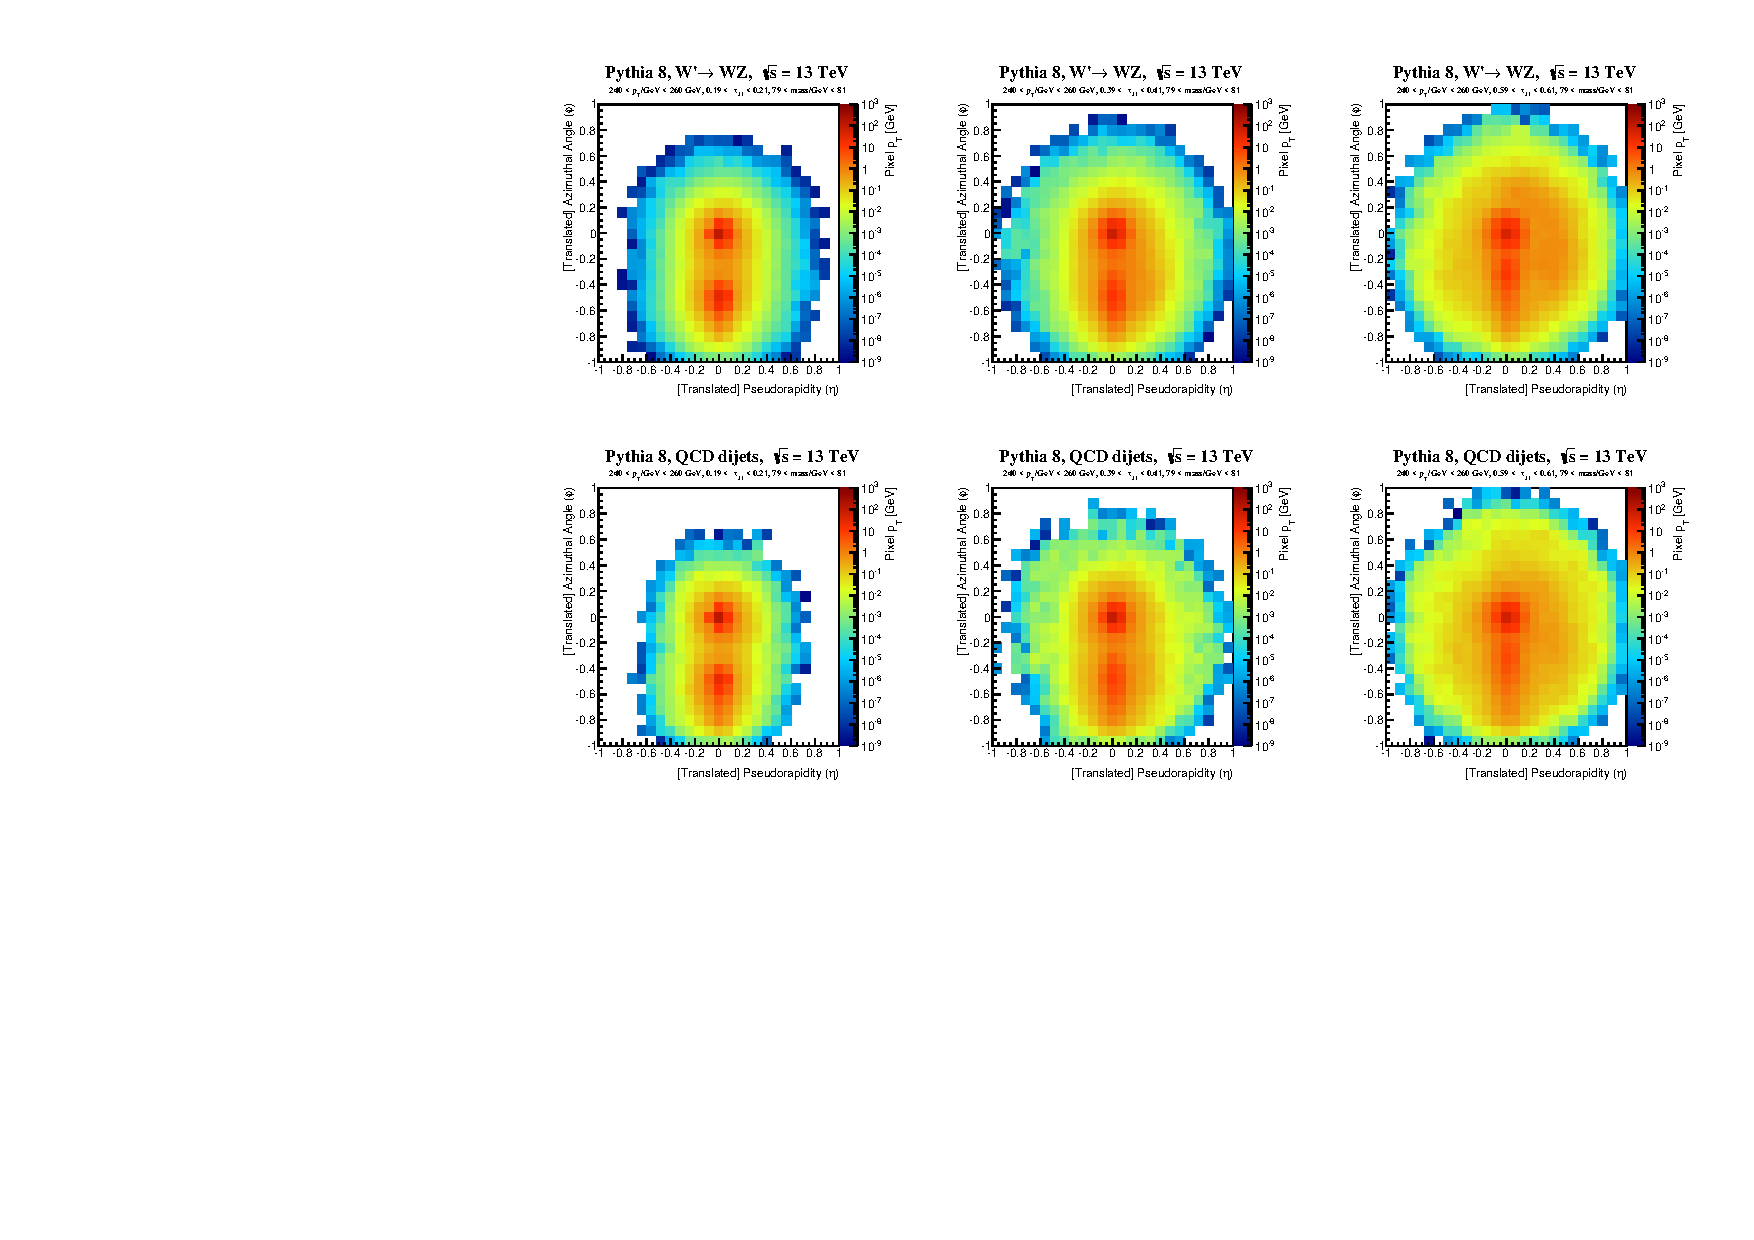
\includegraphics[width=0.99\textwidth]{figures/averages_fixed_nonorm.pdf}
      } \\
      \subfloat[Average image difference \label{subfig:windowdiff}]{
        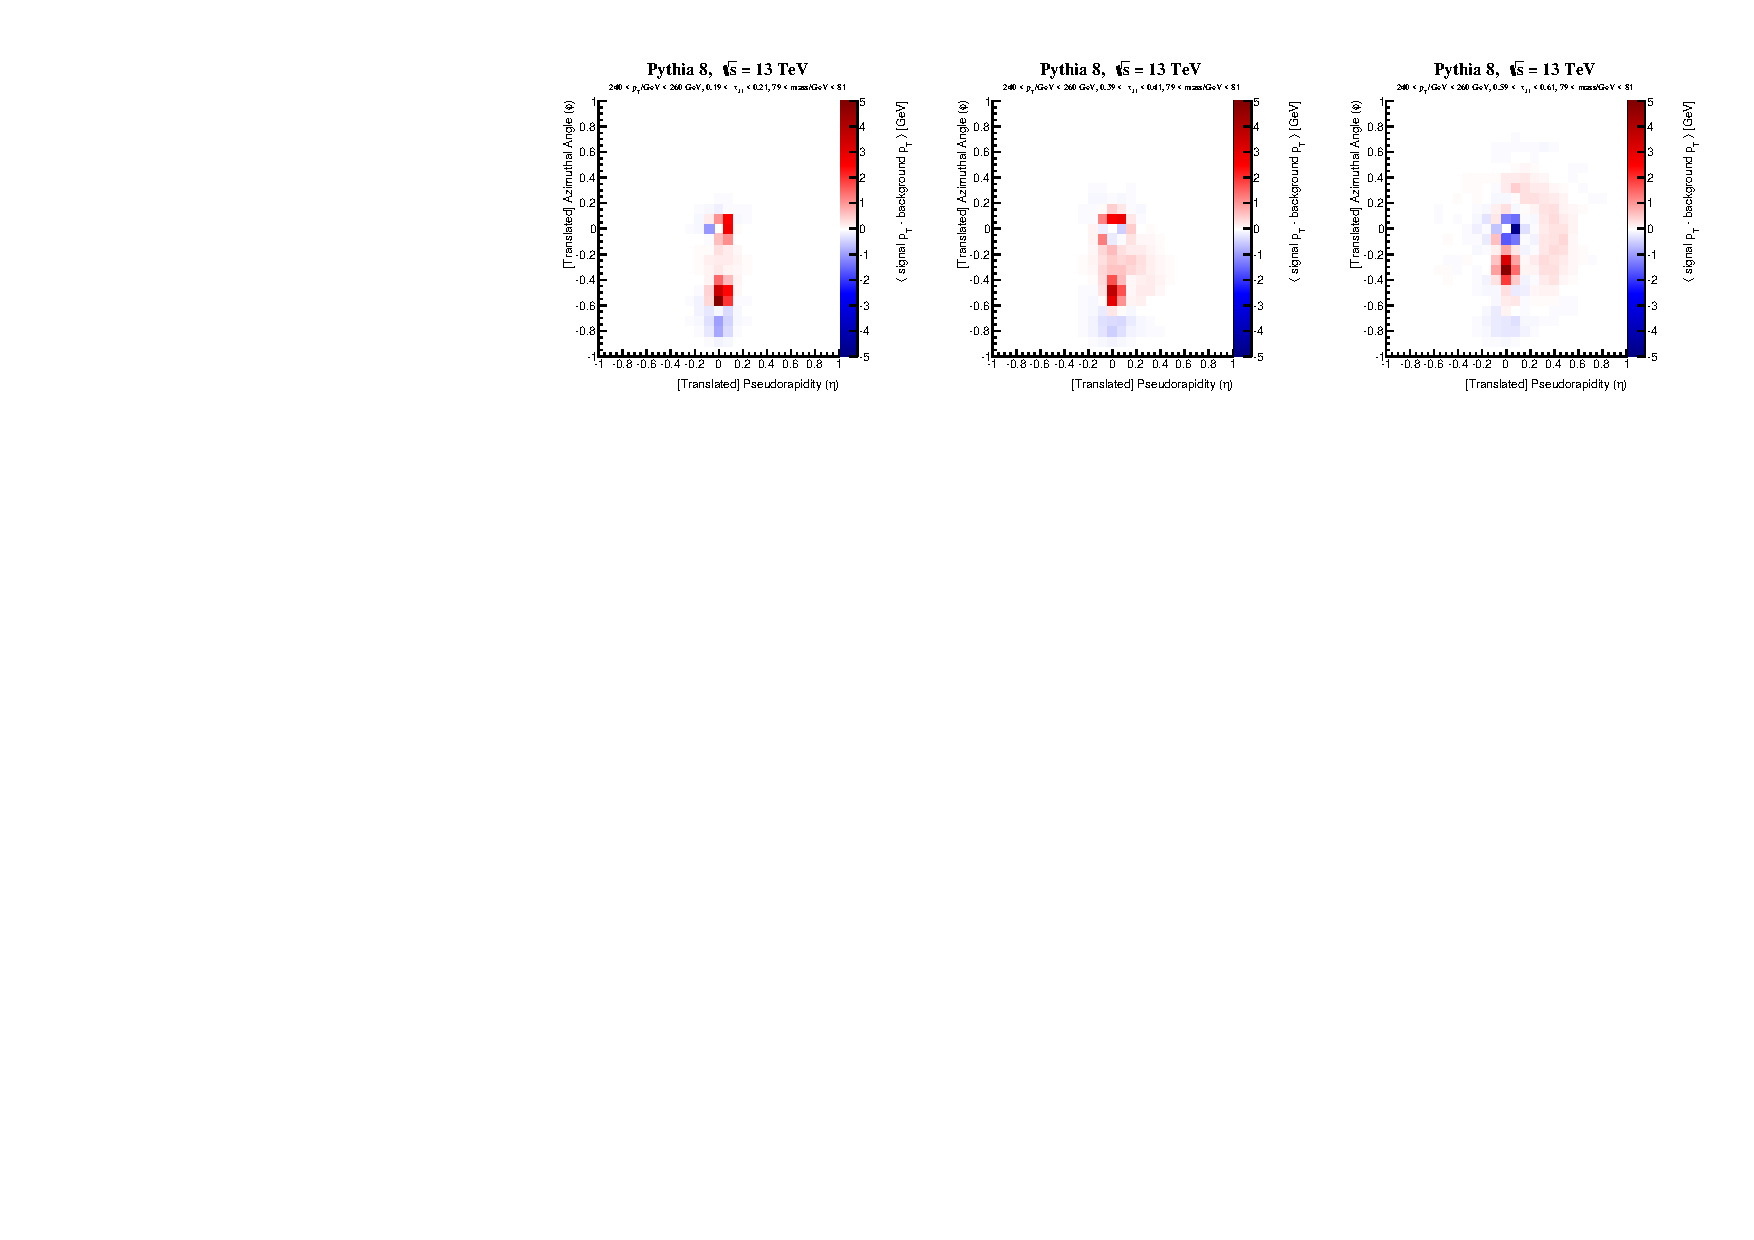
\includegraphics[width=0.99\textwidth]{figures/difference_fixed_nonorm.pdf}
      }
      \caption{
        $W'\rightarrow WZ$ (left) and QCD (right) average jet-images, and Signal - Background image difference (bottom)
        \label{fig:meanImagesWindow} 
      }
    \end{center}
\end{figure}  

\begin{figure}[htbp]
  \centering
  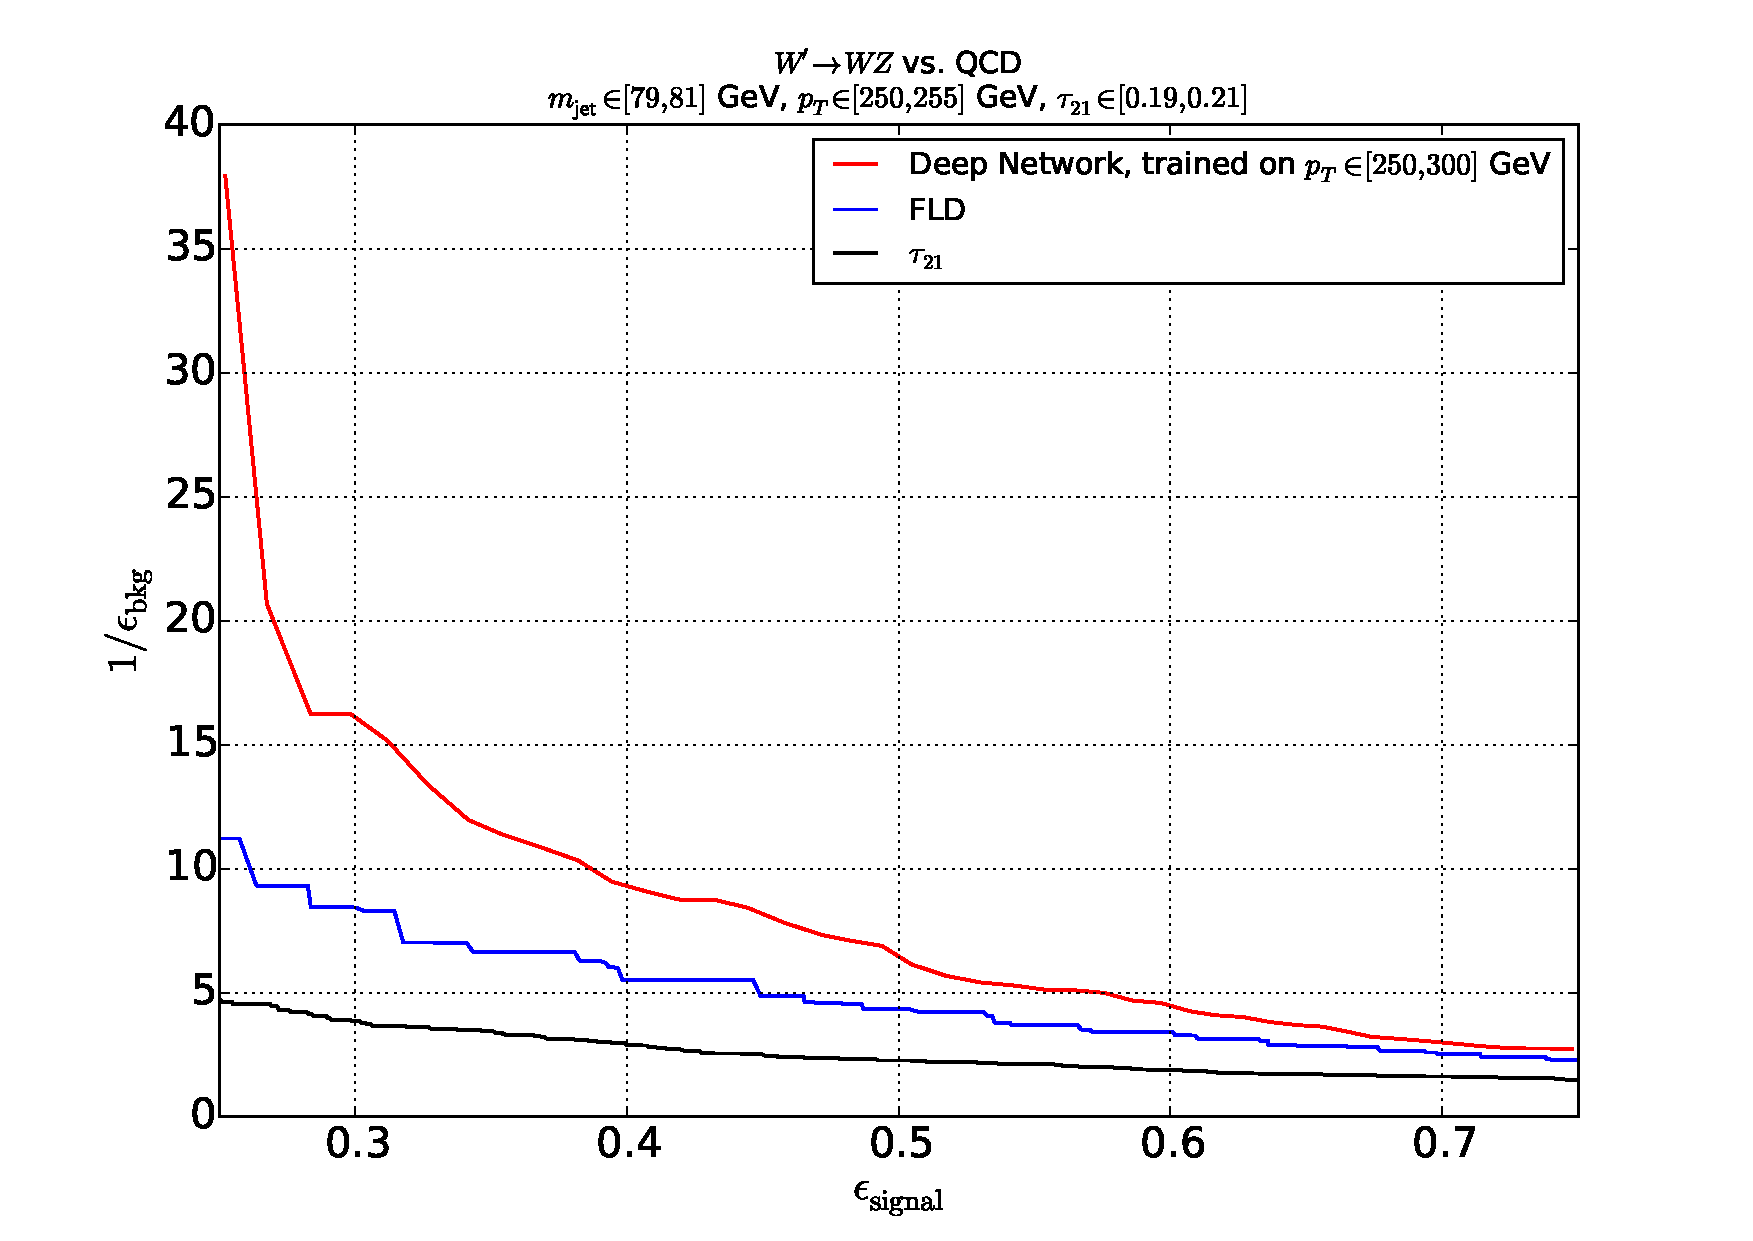
\includegraphics[width=0.95\textwidth]{figures/augwindow-roc.pdf}
  \caption{Receiver Operating Characteristic (ROC) over window sample}
  \label{fig:rocWindow}
\end{figure}

\subsubsection{Understanding what we learn} % (fold)
\label{ssub:understanding_what_we_learn}

\begin{figure}[htbp]
  \centering
  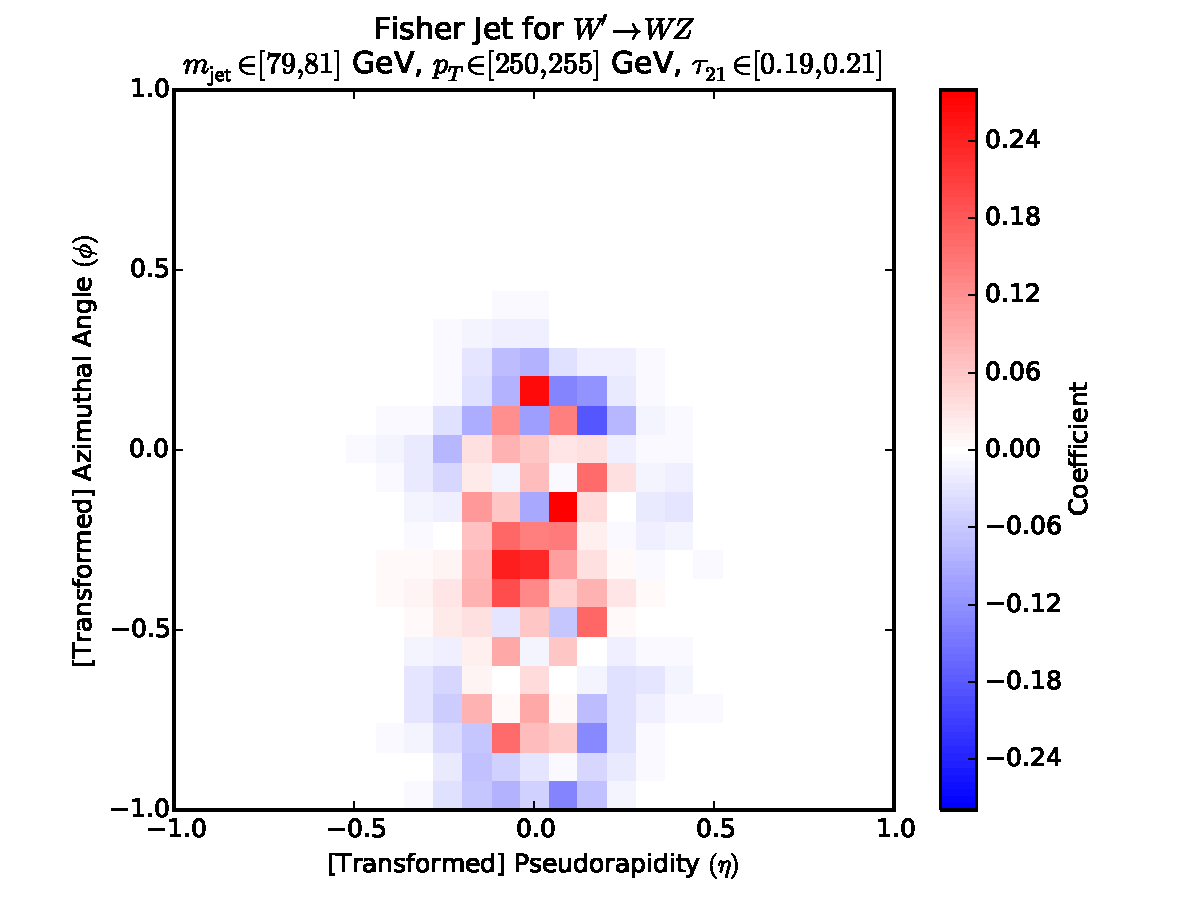
\includegraphics[width=0.65\textwidth]{figures/fld-benwindow.pdf}
  \caption{Cell coefficients from Fisher Linear Discriminant in window: $m_\text{jet}\in [79, 81]$ GeV, $p_{T}\in [250, 255]$ GeV, $\tau_{21}\in[0.19, 0.21]$}
  \label{fig:fldWindow}
\end{figure}

\begin{figure}[htbp]
  \centering
  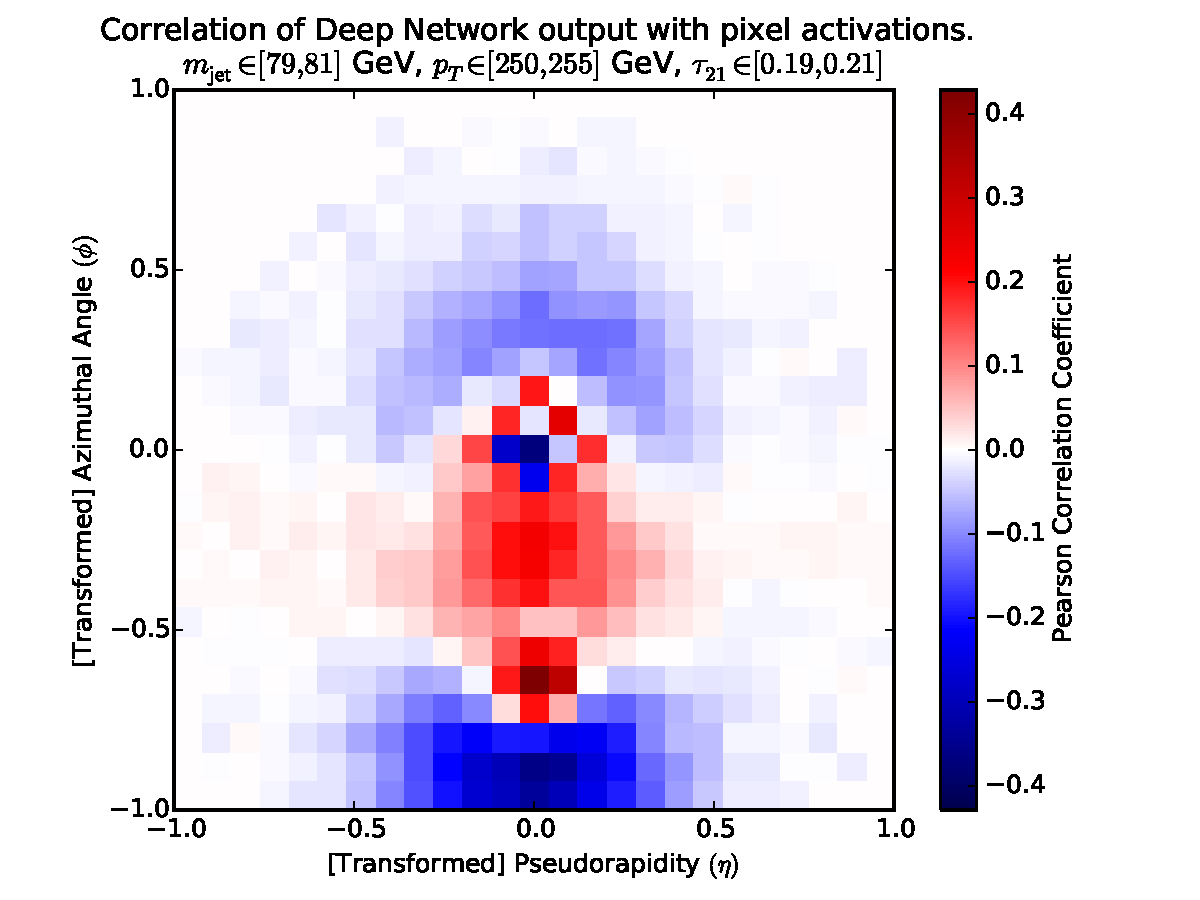
\includegraphics[width=0.65\textwidth]{figures/pixel-activations-corr-benwindow.pdf}
  \caption{Pearson Correlation Coefficient for pixels vs. DNN output, $m_{\mathsf{jet}}\in [79, 81]$ GeV, $p_{T}\in [250, 255]$ GeV, $\tau_{21}\in[0.19, 0.21]$}
  \label{fig:corrWindow}
\end{figure}

%In Figure~\ref{fig:convkernelsWindow}, we show the same feature representations as in Figure~\ref{subfig:convolvedfilters}, which show the convolved differences in images over signal and background in the window. 
%
%\begin{figure}[htbp]
%  \centering
%  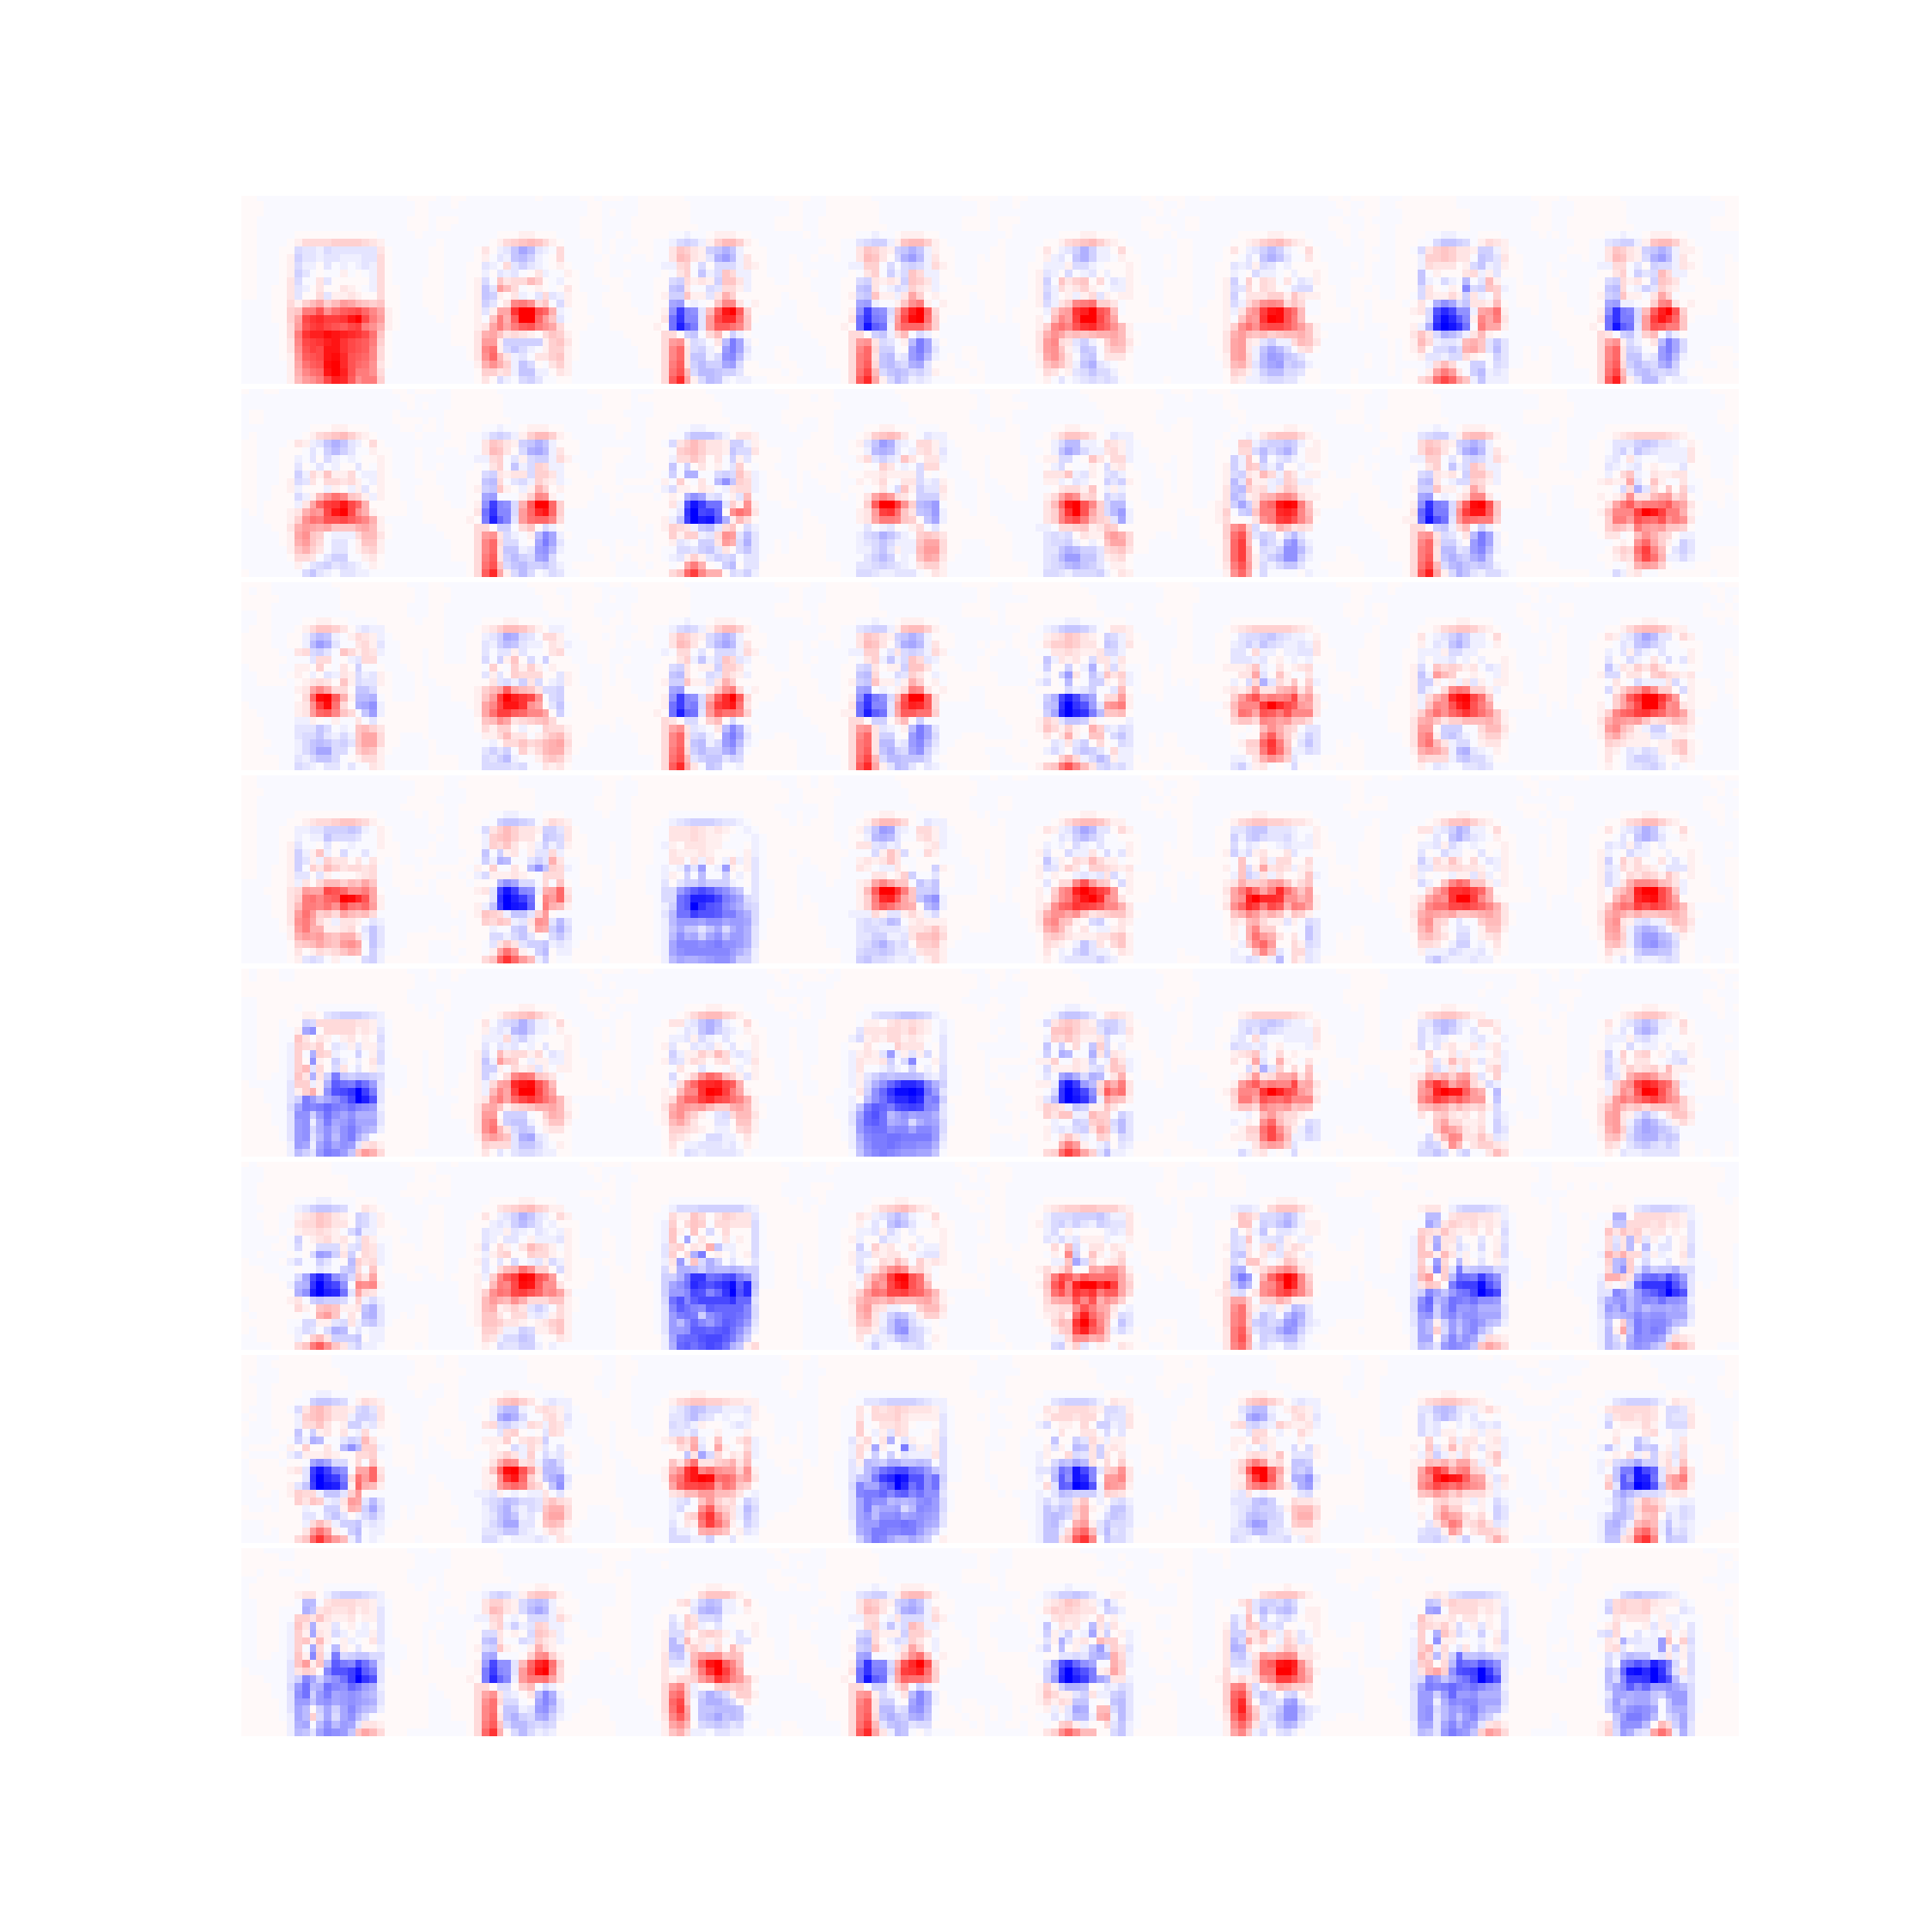
\includegraphics[width=0.95\textwidth]{figures/conv-diffs-ben-window.pdf}
%  \caption{Convolved Feature Differences in jet images, $m_\text{jet}\in [79, 81]$ GeV, $p_{T}\in [250, 255]$ GeV, $\tau_{21}\in[0.19, 0.21]$}
%  \label{fig:convkernelsWindow}
%\end{figure}


% subsubsection understanding_what_we_learn (end)

% subsection small_window_studies (end)

